\newpage
\section{Ganze Zahlen $\mathbb{Z}$}

% ----------------------------------------------------------------------------
\subsection{Definition}

Welche Zahl muss zu Fünf addiert werden, um Null zu erhalten?
\[
  5 + \square = 0
\]
Wenn nur die natürlichen Zahlen betrachtet werden, gibt es keine Antwort auf diese Frage. Wenn in der Mathematik eine Lücke entdeckt wird, dann wird oft etwas neues definiert, das heisst «erfunden», um diese Lücke zu füllen.

In diesem Fall werden neue Zahlen definiert, welche diese Gleichung erfüllen.

\textbf{Definition:} Eine Zahl, welche Null ergibt, wenn sie zu einer gegebenen Zahl $a$ addiert wird, wird \textbf{Gegenzahl} von $a$ genannt und mit $-a$ bezeichnet:
\[
  a + (-a) = 0
\]
Die Gegenzahl von $5$ ist also $-5$ und $5 + (-5) = 0$. Wird die Menge der natürlichen Zahlen um ihre Gegenzahlen erweitert, so ergibt sich die Menge der \textbf{ganzen Zahlen}.

\textbf{Definition:} Die Menge der ganzen Zahlen $\mathbb{Z}$ enthält sämtliche natürliche Zahlen sowie ihre Gegenzahlen.
\[
  \mathbb{Z} = \{\ldots -4, -3, -2, -1, 0, 1, 2, 3, 4, \ldots\}
\]

% ----------------------------------------------------------------------------
\subsection{Zahlengerade und Betrag}

Auch die ganzen Zahlen können auf der Zahlengeraden dargestellt werden. Dabei wird die Gegenzahl jeder Zahl gegenüberliegend der Null dargestellt. So wird die Zahl $-4$ auf der anderen Seite von Null mit gleichem Abstand zur Null wie die Zahl $4$ dargestellt.

\begin{center}
  \begin{tikzpicture}
    \tkzInit[xmin=-5.5,xmax=5.5]
    \tkzDrawX[label={}]
    \tkzLabelX
    \tkzDefPoint(0,0){O}
    \tkzDefPoint(-4,0){A}
    \tkzDefPoint(4,0){B}
    \tkzDrawSegment[dim={$4$,10pt,}](A,O)
    \tkzDrawSegment[dim={$4$,10pt,}](O,B)
  \end{tikzpicture}
\end{center}

Der Abstand einer Zahl $a$ zur Null auf der Zahlengerade wird als ihr Betrag $|a|$ bezeichnet.

\textbf{Definition:} Der \textbf{Betrag} $|a|$ einer negativen Zahl $a$ ist ist die Gegenzahl von $a$. Der Betrag $|a|$ einer nicht-negativen Zahl $a$ ist gleich $a$.
\[
  |a| := \begin{cases}
    a &\quad a \geq 0 \\
    -a &\quad a < 0
  \end{cases}
\]

\begin{example}
  \textbf{Beispiele:} $|-3| = 3 \qquad |4| = 4 \qquad |-4| = 4$
\end{example}

% ----------------------------------------------------------------------------
\subsection{Historisches}

Der indische Mathematiker Brahmagupta, der im 7. Jahrhundert lebte, hat als erster Regeln für das Rechnen mit negativen Zahlen aufgestellt. Er hat die positiven Zahlen «Vermögen» und die negativen «Schulden» genannt.

\begin{minipage}[t]{0.45\textwidth}
  \vspace{0cm}
  \includegraphics[width=.9\textwidth]{Pacioli.jpg}
\end{minipage}
\begin{minipage}[t]{0.55\textwidth}
  \vspace{0cm}
  Im 15. Jahrhundert wurde in Italien die doppelte Buchführung entwickelt. Dabei wurden Schulden als negative Zahlen notiert. Der italienische Mathematiker und Franziskaner Luca Pacioli hat diese Praxis in seinem Werk \textit{Summa de Arithmetica, Geometria, Proportioni et Proportionalità} festgehalten.
\end{minipage}

% ----------------------------------------------------------------------------
\subsection{Abgeschlossenheit}

Die ganzen Zahlen sind bezüglich der folgenden Operationen abgeschlossen:
\begin{itemize}[noitemsep]
  \item Addition
  \item Subtraktion
  \item Multiplikation
\end{itemize}
Das bedeutet, dass die Summe, die Differenz und das Produkt zweier ganzen Zahlen immer eine ganze Zahl ist.

% ----------------------------------------------------------------------------
\subsection{Teilmengen}
Oft wird über bestimmte Teilmengen der ganzen Zahlen gesprochen. Dabei werden die folgenden Begriffe und Symbole verwendet:
\begin{center}
  \renewcommand{\arraystretch}{1.3}
  \begin{tabularx}{0.8\textwidth}{Xcl}
      \textbf{Begriff}           & \textbf{Symbol}  & \textbf{Menge} \\
    \toprule
      positive ganze Zahlen      & $\mathbb{Z}^{+}$   & $\{1, 2, 3, 4, \ldots\}$ \\
    \midrule
      nichtnegative ganze Zahlen & $\mathbb{Z}_{0}^{+}$ & $\{0, 1, 2, 3, 4, \ldots\} = \mathbb{N}$ \\
    \midrule
      negative ganze Zahlen      & $\mathbb{Z}^{-}$   & $\{\ldots, -4, -3, -2, -1 \}$ \\
    \midrule
      nichtpositive ganze Zahlen & $\mathbb{Z}_{0}^{-}$ & $\{\ldots, -4, -3, -2, -1, 0 \}$ \\
    \bottomrule
  \end{tabularx}
\end{center}

% ----------------------------------------------------------------------------
\subsection{Negative und Gegenzahlen}

Es ist wichtig, negative Zahlen und Gegenzahlen zu unterscheiden. Negative Zahlen sind immer Gegenzahlen von positiven Zahlen. Eine positive Zahl kann aber auch eine Gegenzahl sein. So ist beispielsweise $5$ die Gegenzahl von $-5$.

Wenn eine Variable $a$ verwendet wird, um über eine unbekannte Zahl zu sprechen, so kann es sein, dass die Gegenzahl $-a$ eine positive Zahl ist, nämlich wenn $a$ eine negative Zahl ist.

% ----------------------------------------------------------------------------
\subsection{Rechenregeln}

Für das Rechnen mit Gegenzahlen gelten die folgenden Rechenregeln:

\begin{theorem}
  \textbf{Gegen-Gegenzahl.} Die Gegenzahl der Gegenzahl einer Zahl ist die ursprüngliche Zahl:
  \[
    -(-a) = a
  \]
\end{theorem}

\begin{theorem}
  \textbf{Addition und Subtraktion.} Das Addieren der Gegenzahl ist das Gleiche wie das Subtrahieren der Zahl. Das Subtrahieren der Gegenzahl ist das gleiche wie das Addieren der Zahl.
  \[
    a+(-b) = a-b \qquad\qquad a-(-b) = a+b
  \]
\end{theorem}

\begin{theorem}
  \textbf{Subtraktion einer Summe.} Die Subtraktion einer Summe ist das Gleiche wie das Subtrahieren beider Summanden:
  \[
    a-(b+c) = a-b-c
  \]
\end{theorem}

\begin{theorem}
  \textbf{Subtraktion einer Differenz.} Die Subtraktion einer Differenz ist das Gleiche wie das Subtrahieren des Minuenden und das addieren des Subtrahenden.
  \[
    a-(b-c) = a-b+c
  \]
\end{theorem}

\begin{theorem}
  \textbf{Multiplikation von Gegenzahlen.} Für die Multiplikation von Gegenzahlen gelten folgende Regeln:
  \[
    (-a)\cdot b = a\cdot(-b) = -ab \qquad\qquad  (-a)\cdot(-b) = ab
  \]
\end{theorem}
